\section{Data and Results}

\begin{figure}[h]
  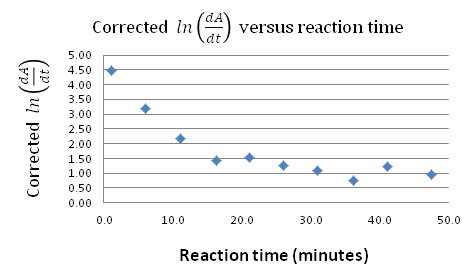
\includegraphics[scale=0.5]{./Figures/20M_dipic_readings.png}\\
  \caption{laksjdf askdfj asdkljfhaslkdjfhaklsdjfh asldkfjhasdlkjfhalksdjfhalksdjfh asldkfjhasdlkfjashdlfkajsdhflkajshdf asdfa sdiufhaisdu fas dfasd fasef asefasef asefas efasefkahsdkjfhaskldjfha sdfasldkfjhasdlfkjasdh falksdjfhalskdjfhasdlkfjah sdflkjashdlkfjah sdlkfjh aslkdjfh aslkdjfhalksdjfhalksjdh flkajsdhf alsdkjfash dflaskdjfah .}\label{fig:0.20M_dipic_readings}
\end{figure}

In the past decade, supervised activity recognition methods have been studied by many researchers, however these methods still face many challenges in real world settings. Supervised activity recognition methods assume that we are provided with labeled training examples from a set of predefined activities. Annotating and hand labeling data is a very time consuming and laborious task. Also, the assumption of consistent pre-defined activities might not hold in reality. More importantly, these algorithms do not take into account the streaming nature of data, or the possibility that the patterns might change over time. In this chapter, we will provide an overview of the state of the art \emph{unsupervised} methods for activity recognition. In particular, we will describe a scalable activity discovery and recognition method for complex large real world datasets, based on sequential data mining and stream data mining methods.

\begin{figure}[h]
  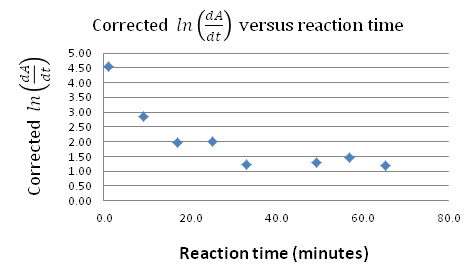
\includegraphics[scale=0.5]{./Figures/10M_dipic_readings.png}\\
  \caption{blahblah.}\label{fig:0.10M_dipic_readings}
\end{figure}

\begin{figure}[h]
  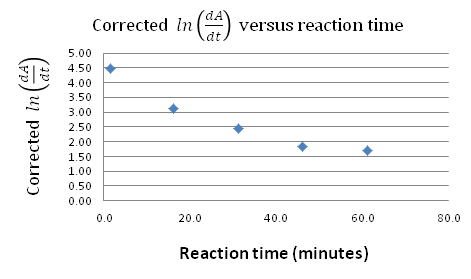
\includegraphics[scale=0.5]{./Figures/05M_dipic_readings.png}\\
  \caption{blahblah.}\label{fig:0.05M_dipic_readings}
\end{figure}

\begin{figure}[h]
  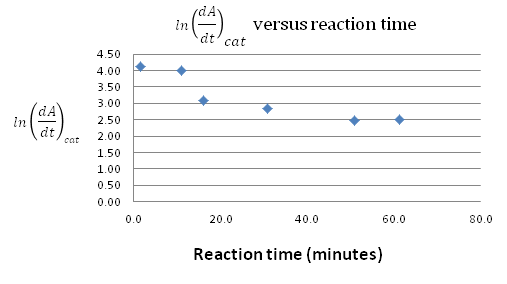
\includegraphics[scale=0.5]{./Figures/032M_dipic_readings.png}\\
  \caption{blahblah.}\label{fig:0.032M_dipic_readings}
\end{figure}

\begin{figure}[h]
  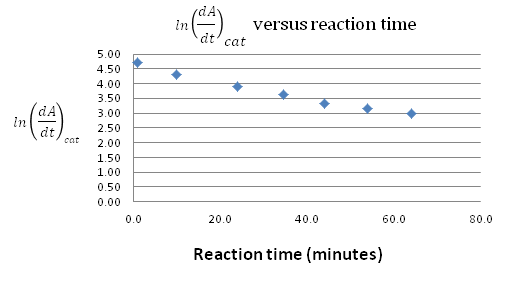
\includegraphics[scale=0.5]{./Figures/016M_dipic_readings.png}\\
  \caption{blahblah.}\label{fig:0.016M_dipic_readings}
\end{figure}

\begin{center}
\begin{table}[h]
    \begin{tabular}{| l | l | l |}
    \hline
    Constant & Empirical Value & Accepted Value \\ \hline
    $K_{EML}$ & $(20\pm{18}){\ }M^{-1}$ & foobar \\ \hline
    $k_{d}$ & $(0.10\pm{0.10}){\ }mins^{-1}$ & blah \\ 
    \hline
    \end{tabular}
    \caption[Table caption text]{Values of $K_{EML}$ and $k_d$, as determined in this experiment as well as accepted values from literature}
    \label{tbl:summary}
\end{table}
\end{center}